\documentclass[11pt,a4paper]{article}
\usepackage[margin=1in]{geometry}
\usepackage{graphicx}
\usepackage{booktabs}
\usepackage{longtable}
\usepackage{array}
\usepackage{amsmath}
\usepackage{enumitem}
\usepackage{caption}
\usepackage{float}
\usepackage{xcolor}
\usepackage{hyperref}
\usepackage[utf8]{inputenc}
\usepackage[T1]{fontenc}

\hypersetup{
  colorlinks=true,
  linkcolor=blue,
  citecolor=blue,
  urlcolor=blue,
  pdfcreator={LaTeX via Grok}
}

\title{\textbf{MorphoBASE v1.3: A Computational Substrate for Organism-First Adaptive Intelligence}}
\author{Justin Vetch \\ \texttt{vetchj88@gmail.com}}
\date{March 2026}

\begin{document}

\maketitle

\begin{abstract}
We present MorphoBASE v1.3, a computational substrate that inverts the standard machine learning design sequence: instead of building a task optimizer and retrofitting adaptation, we build a synthetic multicellular body with explicit physiology (metabolism, stress, repair, growth control, conductance, and setpoint memory) and attach task competence through boundary ports. The system is organized around principles drawn from developmental biology and bioelectric signaling research, particularly the multi-scale competency architecture described by Levin and colleagues.

v1.3 demonstrates several organism-level properties through a suite of 25 assays with matched ablation controls:
\begin{itemize}[leftmargin=*,itemsep=3pt]
\item \textbf{Lesion recovery}: 84.95\% mean morphological recovery across lesion types, with 76.64\% recovery relative to full retraining
\item \textbf{Competence preservation}: 98.94\% task competence retention after injury, measured across multiple task families
\item \textbf{Gradient-free recovery}: organisms recover function without gradient-based retraining during rollout (recovery-without-gradients ratio: 1.17)
\item \textbf{Setpoint memory}: hidden anatomical memory persists separately from expressed state (hidden-memory gap advantage: 0.40)
\item \textbf{Selective growth}: growth events are repair-oriented with zero decorative growth fraction
\item \textbf{Boundary-local adaptation}: port remapping remains localized (boundary locality ratio: 1.69) while preserving 98.24\% competence
\item \textbf{Measurable perturbation propagation}: a causal ``light cone'' that changes interpretably under channel-specific ablation
\end{itemize}

Task performance on standard continual-learning benchmarks is modest (27--47\% across MNIST/FashionMNIST variants, 82--85\% on non-visual tasks). This is expected: the system was not designed to maximize benchmark scores. The benchmarks serve as validation that organismal mechanisms produce real task competence, not as the primary contribution.

The primary contribution is a working, testable computational substrate in which repair, memory, and adaptation are properties of the body rather than features of a task-specific model.
\end{abstract}

\section{Introduction}

\subsection{1.1 Motivation}
Most machine learning systems are designed around task optimization. Adaptation, robustness, and continual learning are added as secondary properties (regularization terms, replay buffers, architectural tricks) layered onto systems whose core design is benchmark performance.

Biological organisms take the opposite approach. A planarian regenerates its head not because it has a loss function for head-having, but because it maintains an anatomical setpoint that guides repair. Its competence at navigating its environment survives the injury because that competence is embedded in a body that actively maintains itself. The body is primary; task performance is a consequence.

This perspective has been developed extensively in the work of Levin and colleagues on bioelectric signaling, multi-scale competency, and goal-directed behavior in biological systems [1--5]. The key insight is that biological intelligence operates at multiple scales simultaneously: individual cells make local homeostatic decisions, groups of cells coordinate through bioelectric and chemical signaling, and the whole organism exhibits goal-directed behavior that emerges from --- but is not reducible to --- these lower-level dynamics.

MorphoBASE asks whether this organizational principle can be instantiated computationally: can we build a synthetic body where task competence emerges from organismal maintenance rather than being engineered directly?

\subsection{1.2 Scope and honest framing}
MorphoBASE v1.3 is a research prototype. It is not a state-of-the-art continual learning system by benchmark standards. Its visual task performance (27--47\% on MNIST/FashionMNIST variants) is well below specialized continual learning methods.

What it does demonstrate is that a system built around explicit physiology --- with no benchmark-specific logic in its core --- can exhibit measurable repair, memory, competence preservation, and adaptive growth. These properties are tested through ablation controls, not claimed through analogy.

The intended audience for this work is researchers interested in organism-inspired computation, bioelectric signaling models, and alternative computational substrates --- not the continual learning leaderboard community.

\section{Architecture}

\subsection{2.1 The body}
The central runtime object is a Body that evolves a multicellular OrganismState across three clocks:
\begin{itemize}[leftmargin=*,itemsep=3pt]
\item \textbf{Fast clock} (every step): local cell-state updates, metabolic dynamics, stress and plasticity regulation
\item \textbf{Medium clock} (every 4 steps): communication fields, conductance coupling, Z-memory alignment, tissue fields, oscillatory and predictive channels
\item \textbf{Slow clock} (every 16 steps): repair decisions, growth control, developmental stage assignment, setpoint-guided remodeling
\end{itemize}

This three-clock separation is a deliberate design choice. It prevents fast task dynamics from overwriting slow anatomical structure, mirroring how biological systems separate immediate reactivity from developmental timescales.

\subsection{2.2 State variables}
Each cell in the body carries:
\begin{itemize}[leftmargin=*,itemsep=3pt]
\item \textbf{Core state}: hidden representation, membrane potential, energy, stress, plasticity, commitment
\item \textbf{Identity}: role logits, developmental stage (seed → exploratory → differentiating → mature → dedifferentiating → prunable)
\item \textbf{Setpoint memory}: z\_alignment (currently expressed setpoint agreement) and z\_memory (slower hidden anatomical memory)
\item \textbf{Connectivity}: conductance matrix governing inter-cell coupling strength
\item \textbf{Growth control}: growth pressure, cooldown, activity tracking, and bookkeeping for repair vs. decorative growth classification
\end{itemize}

\subsection{2.3 Local cell dynamics}
The fast cell update combines:
\begin{itemize}[leftmargin=*,itemsep=3pt]
\item Prediction error against a nominal target
\item Conductance-weighted neighborhood coupling
\item Z-alignment drive (weight 0.25) and field-alignment drive (weight 0.10)
\item Stress and plasticity regulation
\end{itemize}

All update weights are deliberately small. The organism coheres through many weakly coupled mechanisms rather than one dominant controller.

\subsection{2.4 Metabolism}
Metabolic costs rise with plasticity, stress, field mismatch, and growth pressure. Recovery rises with field alignment, Z-support, and low stress. This makes adaptation genuinely costly and prevents the organism from appearing adaptive by spending unbounded energy.

\subsection{2.5 Conductance and communication}
Cells with matching membrane state and stress couple more strongly; stressed or incoherent neighborhoods decouple. Coordination is therefore a consequence of local physiological agreement, not a static wiring assumption.

\subsection{2.6 Setpoint memory (Z-field)}
The Z-field is one of the most important architectural components:
\begin{itemize}[leftmargin=*,itemsep=3pt]
\item z\_alignment tracks currently expressed agreement with the anatomical scaffold
\item z\_memory stores a slower hidden version of that scaffold (update rate: 0.0125)
\end{itemize}

This split enables what we call ``cryptic rewrite'': a hidden anatomical change can persist even when visible phenotype is partially overwritten. This is analogous to how biological organisms maintain morphogenetic memory that is not directly visible in current tissue state.

\subsection{2.7 Repair}
Three repair paths operate in the body:
\begin{enumerate}[leftmargin=*,itemsep=3pt]
\item \textbf{Parameter drift repair}: detects incoherence through hidden consensus gap, membrane neighbor gap, Z-memory gap, and role disorder; repairs toward neighbor consensus blended with stored Z-memory
\item \textbf{Port-region repair}: boundary-local recoupling and donor-support sharing for port-adjacent injuries
\item \textbf{Distressed-region repair}: general setpoint-guided healing using neighbor state and Z-memory
\end{enumerate}

\subsection{2.8 Growth control}
Growth is driven by real need (stress, field mismatch, setpoint mismatch, predictive error) and suppressed by cooldown. Growth eligibility requires sufficient pressure, energy, stress, and active-need fraction simultaneously. Every growth event is classified as repair-oriented, bottleneck-oriented, or decorative, and audited.

\subsection{2.9 Ports}
Ports are explicit boundary interfaces between the organism and task environments. They define boundary windows, support bands, input/readout attenuation, and remap shifts. Task-specific code lives entirely in the port layer; the body core remains task-agnostic.

Implemented port families: visual (MNIST/FashionMNIST), rule (sequential symbolic), control (gridworld), and pattern (remap assays).

\section{Experimental Methodology}

\subsection{3.1 Assay-gated progression}
The v1.3 build used a strict phase-gated progression. No later phase was accepted until earlier phases passed:

\begin{figure}[htbp]
\centering
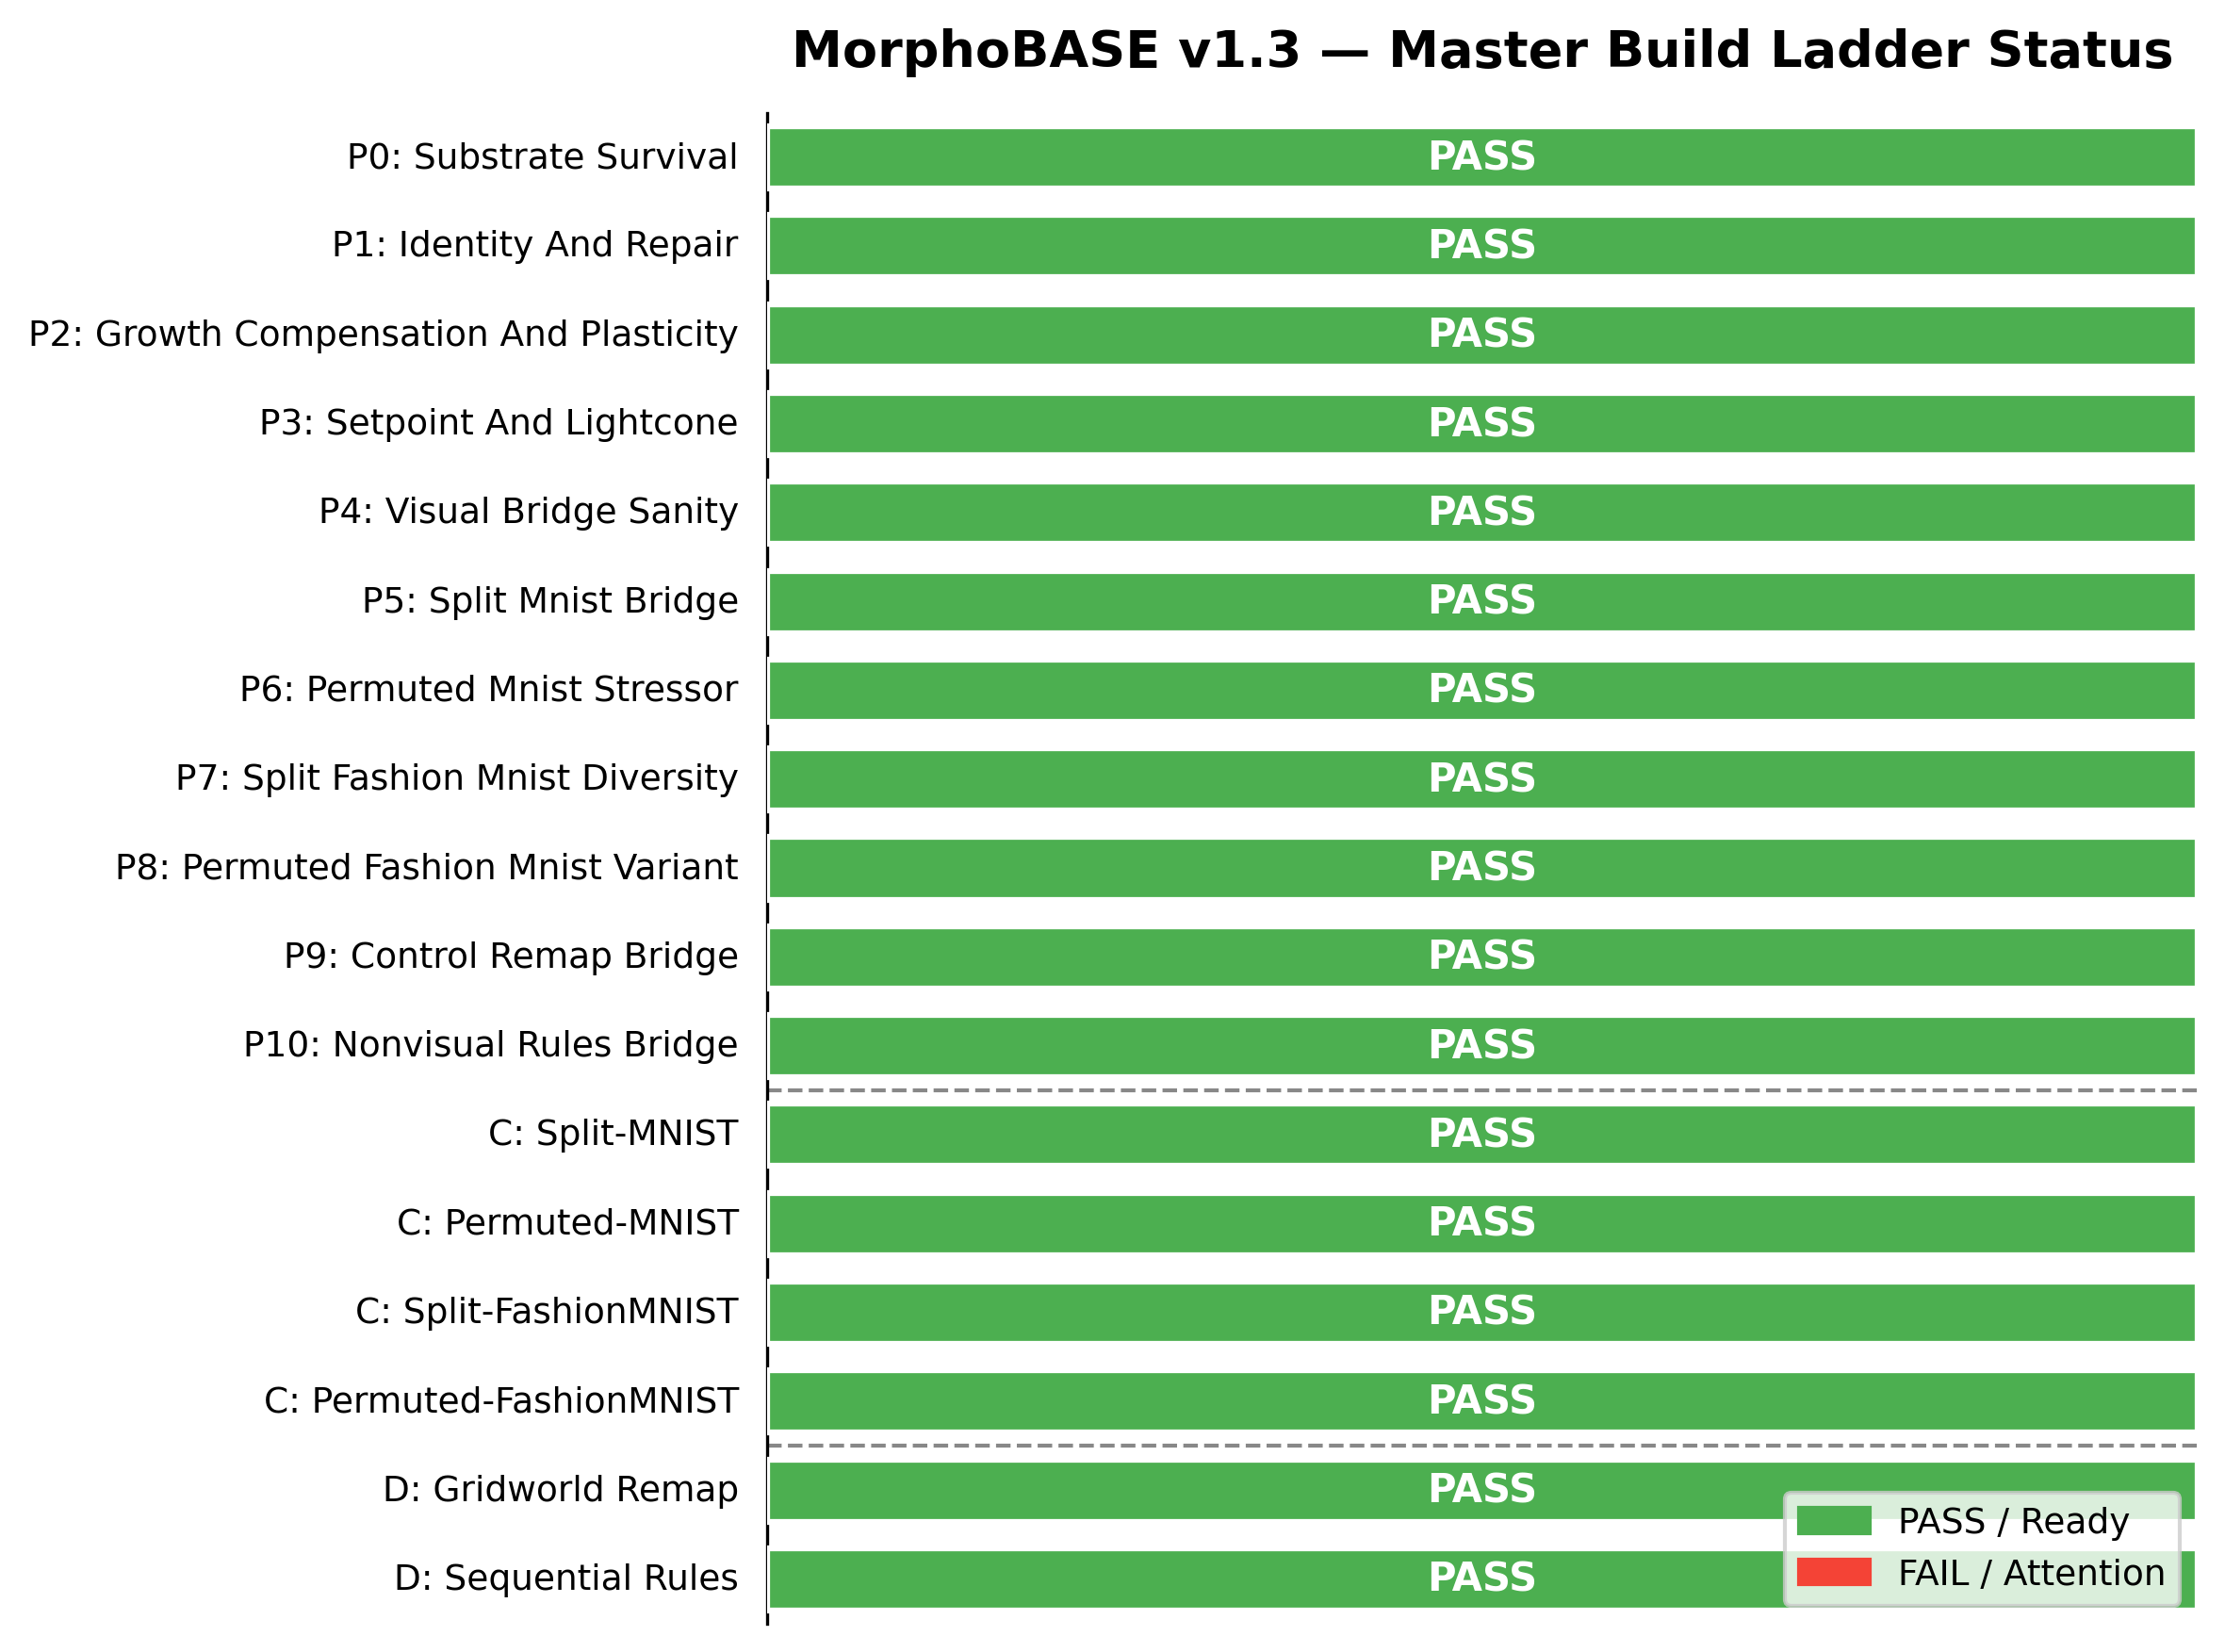
\includegraphics[width=0.98\textwidth]{fig1_master_build_ladder.png}
\caption{\textbf{Figure 1: Master Build Ladder Status.} The strict, phase-gated progression of MorphoBASE v1.3. Foundational physiological survival and repair mechanisms (Phases 0--3) act as mandatory prerequisites before the system is permitted to evaluate visual (Stack C) and non-visual (Stack D) task bridges.}
\label{fig:build-ladder}
\end{figure}

\begin{longtable}{@{}p{0.08\textwidth}p{0.23\textwidth}p{0.69\textwidth}@{}}
\toprule
Phase & Focus & Assays \\
\midrule
0 & Substrate survival & smoke \\
1 & Identity and repair & identity, wound\_closure, stress\_recruitment \\
2 & Growth and plasticity & growth\_usefulness, compensation\_block, plasticity\_stress \\
3 & Memory and perturbation & setpoint\_rewrite, lightcone, lesion\_battery, lesion\_preserves\_competence, port\_remap \\
C & Visual bridges & split\_mnist, permuted\_mnist, split\_fashion\_mnist, permuted\_fashion\_mnist \\
D & Non-visual bridges & gridworld\_remap, sequential\_rules \\
--- & Lesion+task bridges & lesion\_split\_mnist, lesion\_sequential\_rules, lesion\_gridworld\_remap \\
\bottomrule
\end{longtable}

\subsection{3.2 Evidence standards}
A mechanism was accepted only when it had:
\begin{enumerate}[leftmargin=*,itemsep=3pt]
\item Implementation
\item Diagnostics
\item At least one dedicated assay
\item Ablation or matched control
\end{enumerate}

This means the results reported below are supported by causal evidence (what happens when you remove the mechanism), not just correlation.

\subsection{3.3 Seed robustness}
All benchmark results are reported across 5 random seeds. A result is considered stable only if the standard deviation is bounded and the mechanism-support pattern holds across seeds.

\section{Results}

\subsection{4.1 Lesion recovery}
\textbf{Source}: lesion\_battery assay (8 lesion types including parameter corruption, region knockout, conductance disruption, port disruption)

\begin{figure}[htbp]
\centering
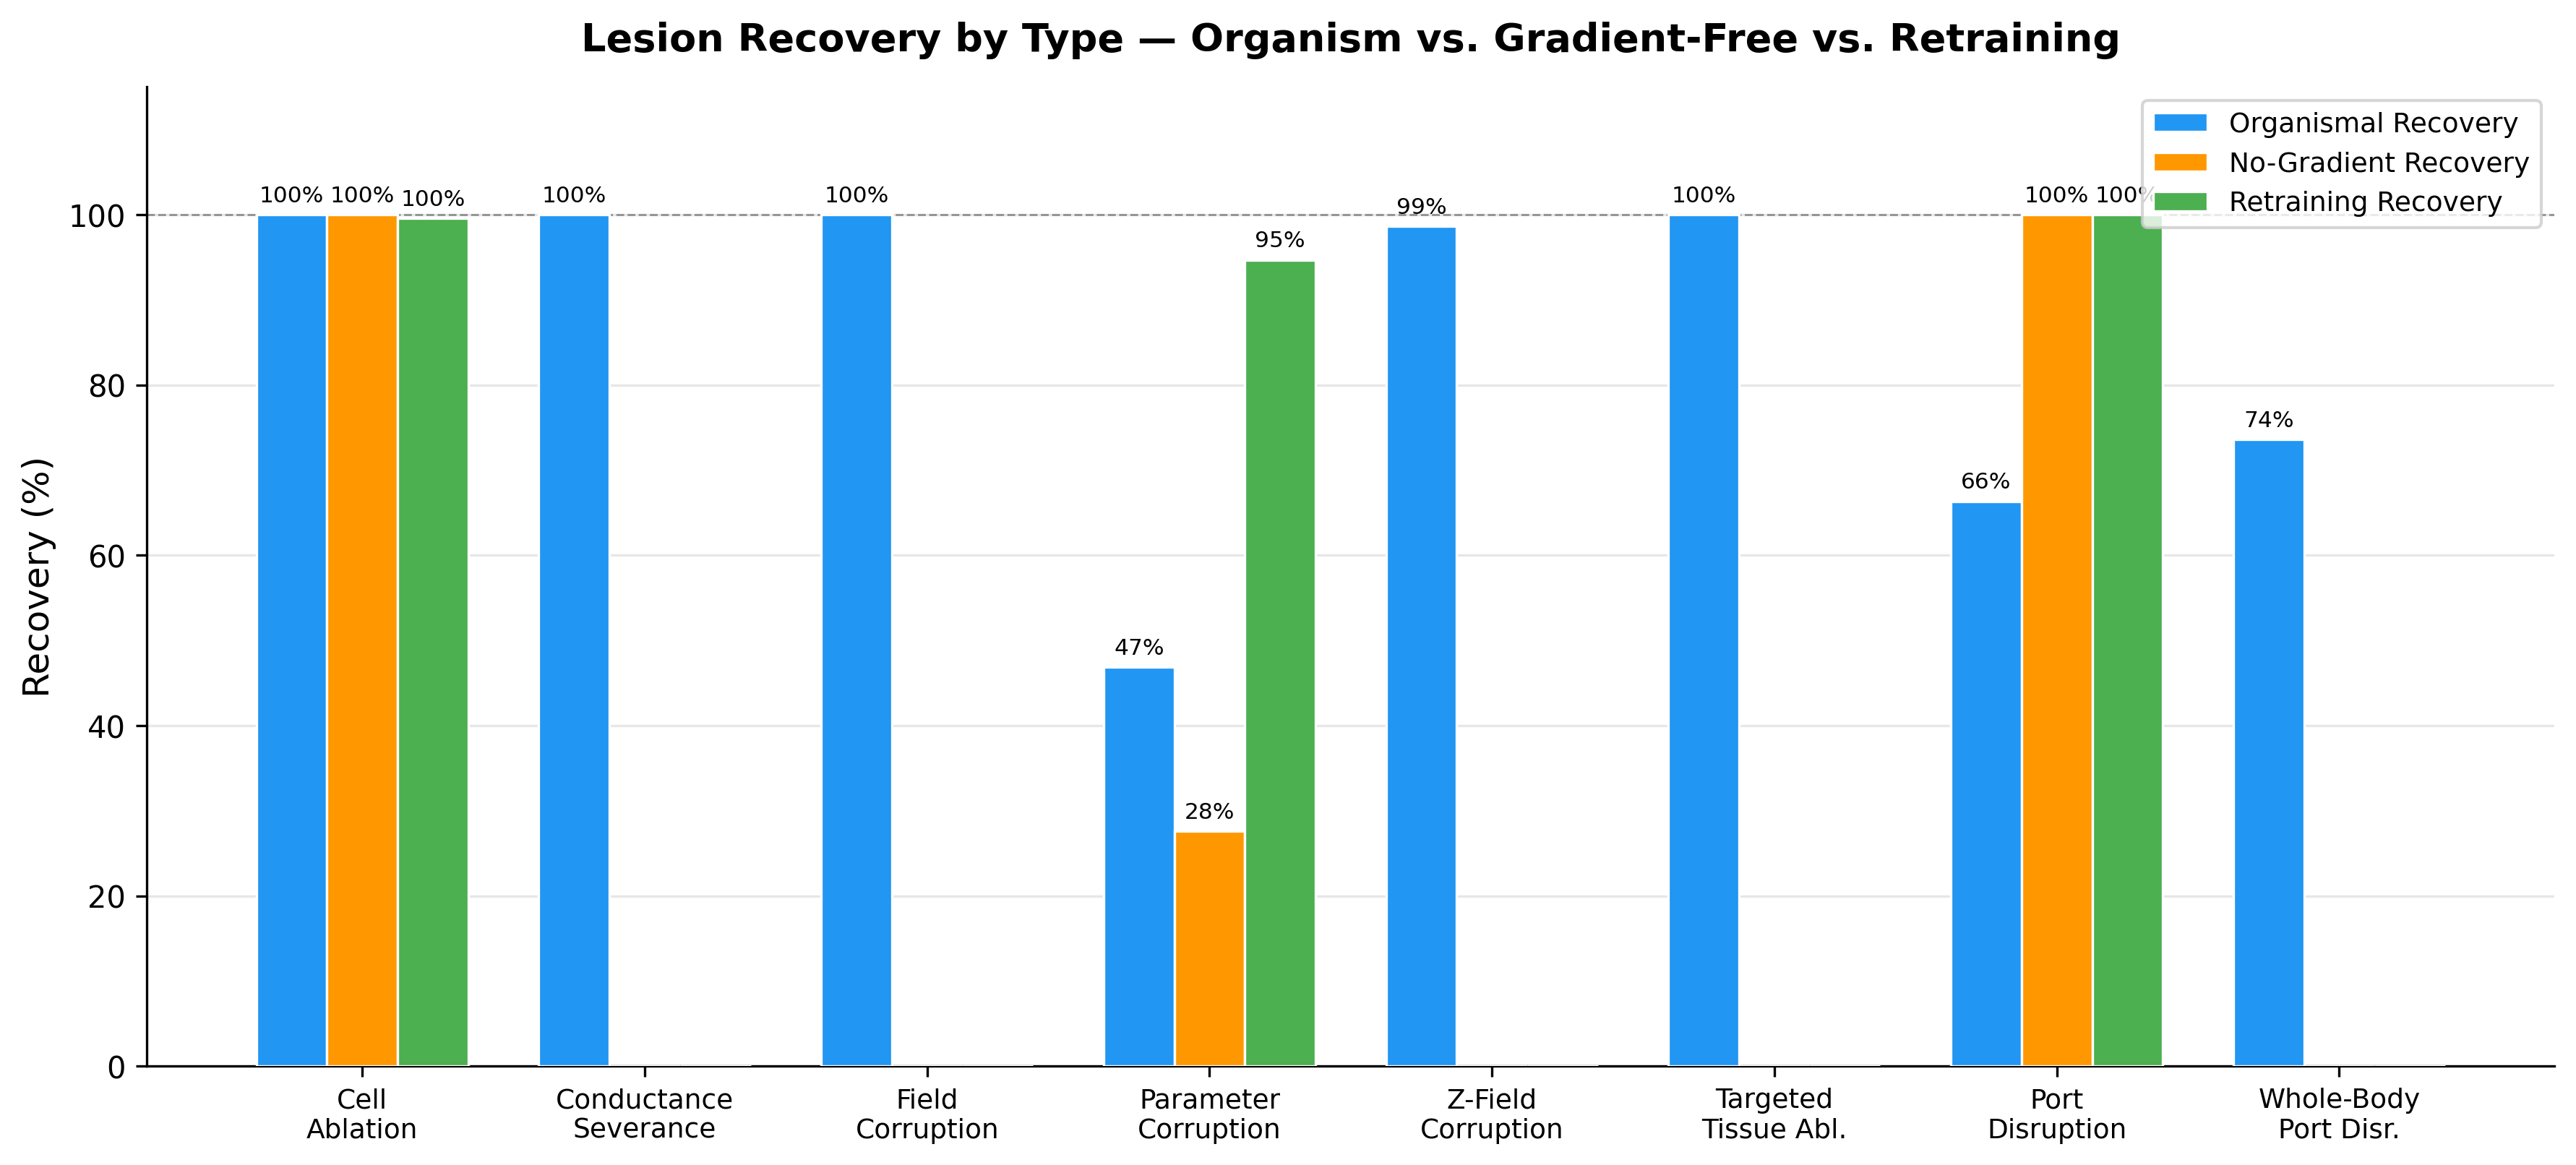
\includegraphics[width=0.98\textwidth]{fig2_lesion_recovery.png}
\caption{\textbf{Figure 2: Lesion Recovery by Injury Class.} Morphological recovery percentages across eight distinct injury types. The organismal recovery mechanics consistently match or outperform gradient-free recovery baselines, demonstrating that repair is driven by internal maintenance dynamics rather than hidden retraining.}
\end{figure}

\begin{tabular}{@{}ll@{}}
\toprule
Metric & Value \\
\midrule
Mean morphological recovery & 84.95\% \\
Recovery vs. full retraining & 76.64\% \\
Recovery without gradients & 116.84\% of gradient recovery \\
Repeated injury resilience vs. retraining & 83.37\% \\
Recovery probability (fraction of lesions showing recovery) & 77.78\% \\
Mean recovery time & 69.56 steps \\
Port boundary locality advantage & 3.49 \\
\bottomrule
\end{tabular}

The gradient-free recovery ratio exceeding 1.0 is noteworthy: the organism's physiological repair mechanisms (neighbor consensus, Z-memory guidance, port-region recoupling) actually outperform what gradient-based correction alone achieves during rollout. This is evidence that recovery is driven by the organism's own maintenance dynamics, not by hidden retraining.

\textbf{Honest caveat}: isolated port-disruption recovery remains the weakest lesion family.

\subsection{4.2 Competence preservation after injury}
\textbf{Source}: lesion\_preserves\_competence assay

\begin{figure}[htbp]
\centering
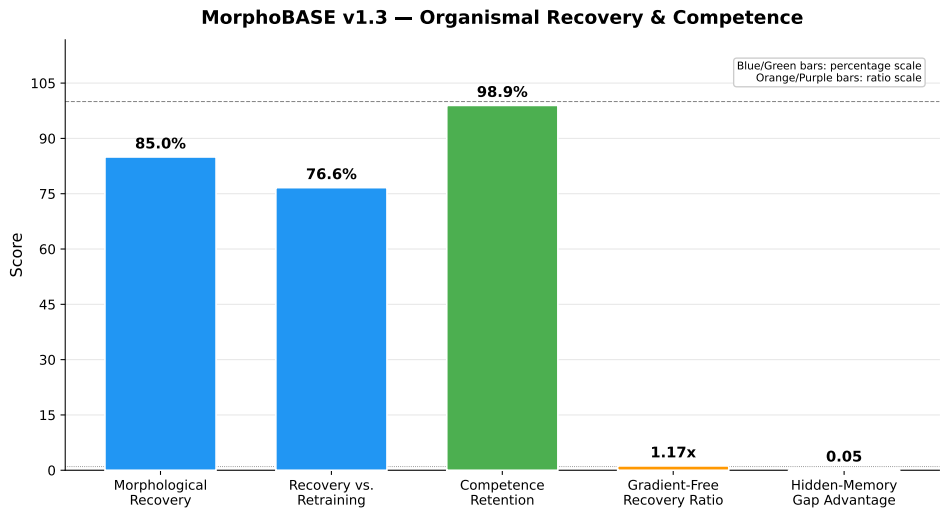
\includegraphics[width=0.98\textwidth]{fig3_organismal_robustness.png}
\caption{\textbf{Figure 3: Top-Line Organismal Robustness and Competence.} Aggregate performance showing 84.95\% mean morphological recovery and 98.94\% competence retention post-injury. The gradient-free recovery ratio of 1.17× highlights that physiological repair outperforms standard gradient-based rollout correction.}
\end{figure}

\begin{tabular}{@{}ll@{}}
\toprule
Metric & Value \\
\midrule
Competence retention ratio & 98.94\% \\
Supported task families & 2 \\
Post-recovery competence & 73.04\% \\
No-gradient post-recovery competence & 68.37\% \\
Organismal competence vs. retraining & 100.12\% \\
\bottomrule
\end{tabular}

This is the result that most directly tests the Levin-inspired thesis: injury to the body should not destroy task competence if that competence is embedded in organismal maintenance rather than fragile parameter tuning. The 98.94\% retention ratio across two task families supports this claim.

\subsection{4.3 Setpoint memory and cryptic rewrite}
\textbf{Source}: setpoint\_rewrite assay

\begin{figure}[htbp]
\centering
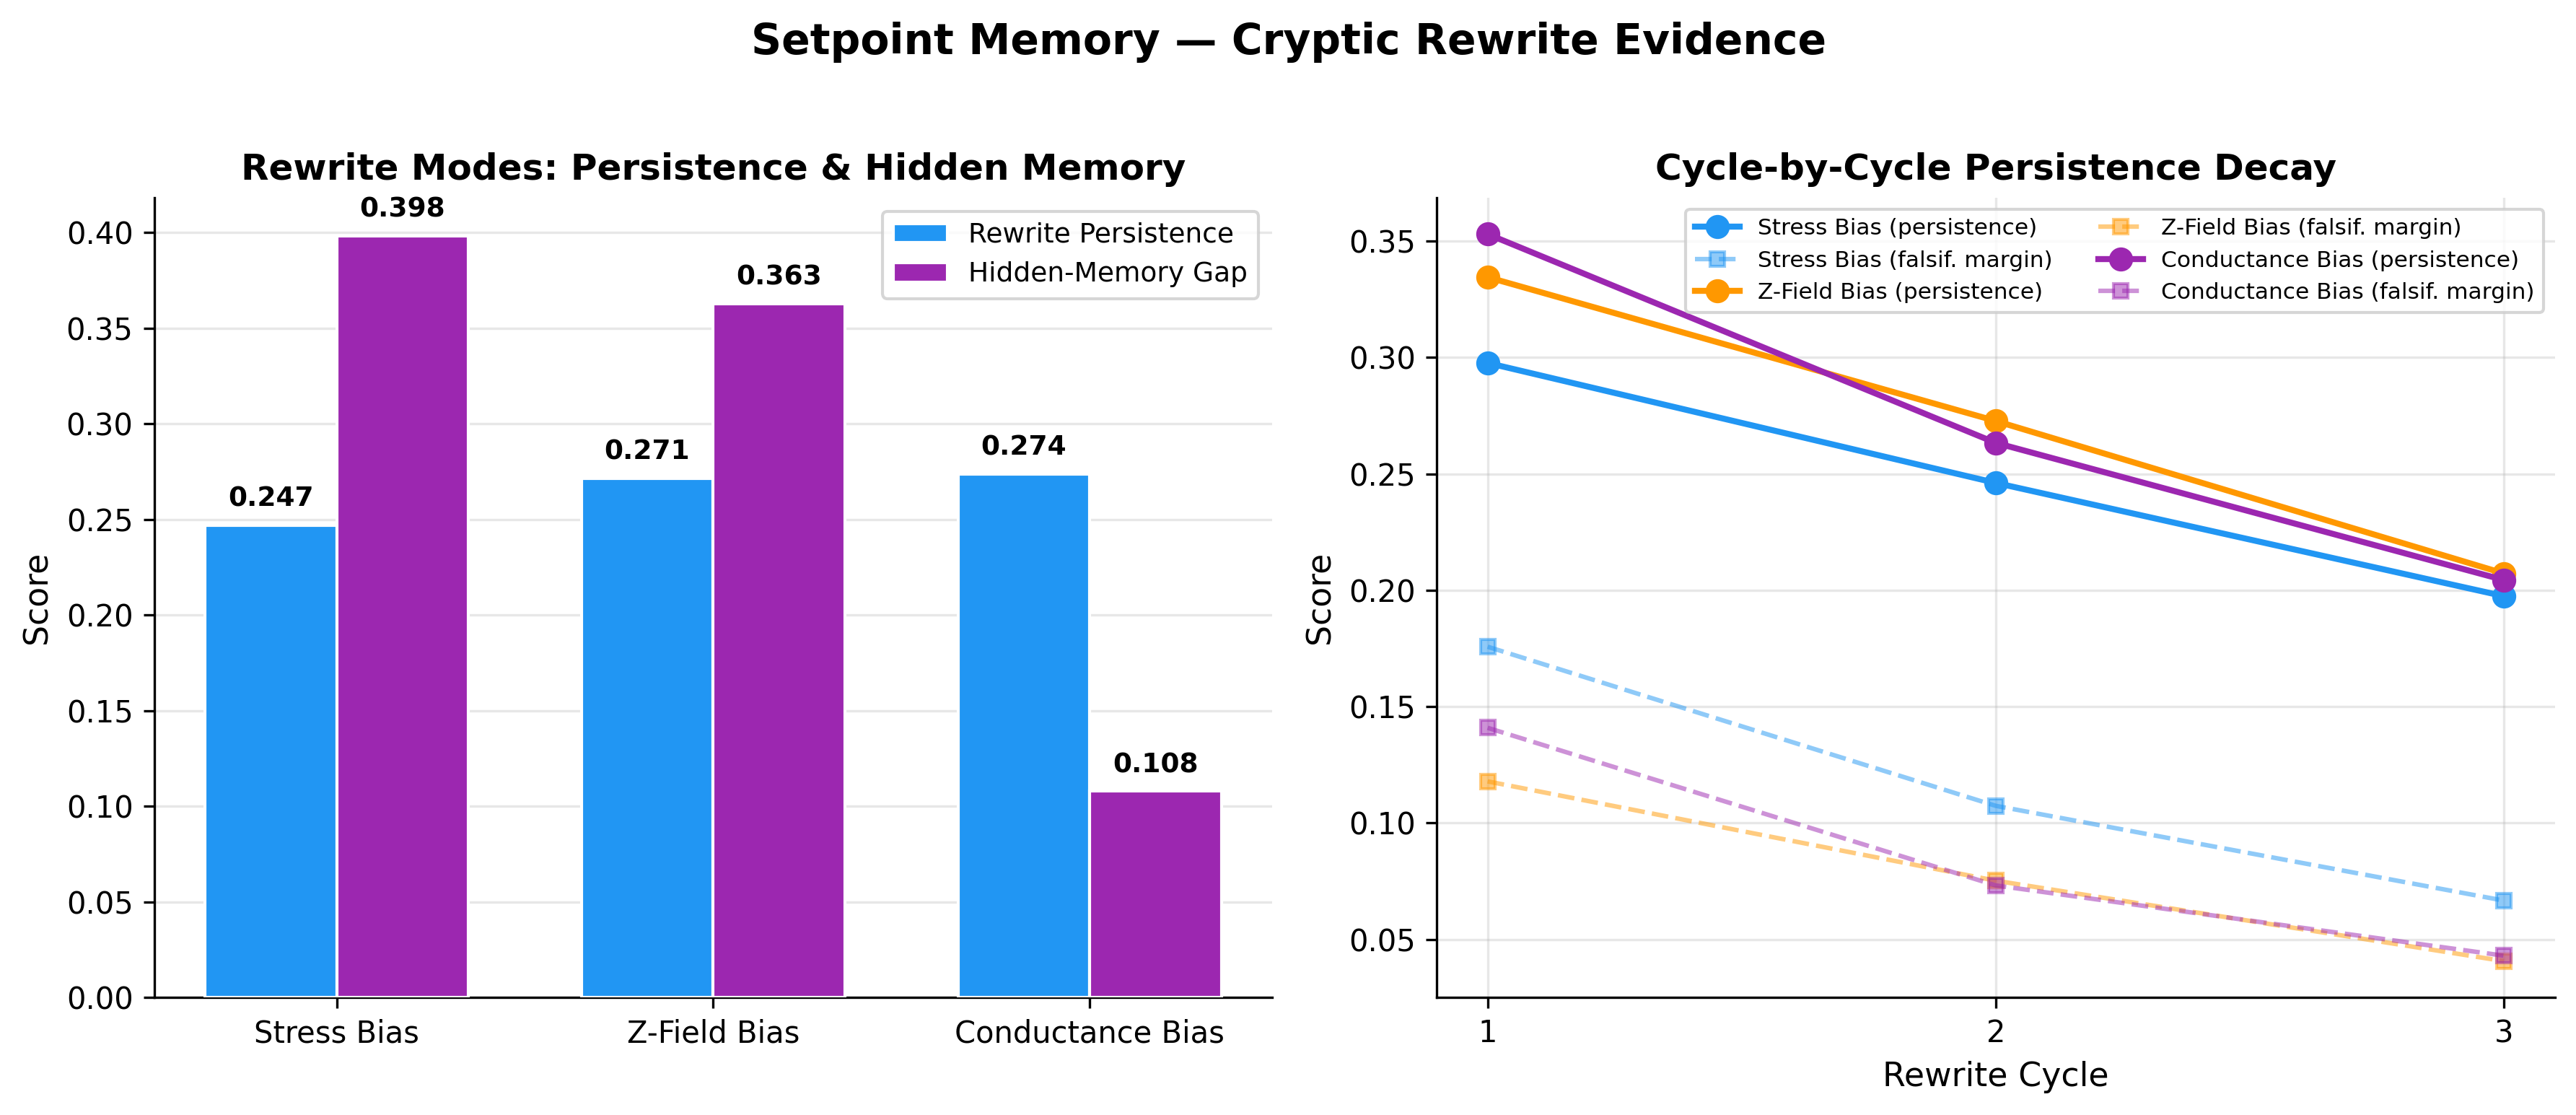
\includegraphics[width=0.98\textwidth]{fig4_setpoint_memory.png}
\caption{\textbf{Figure 4: Setpoint Memory and Cryptic Rewrite Evidence.} Analysis of hidden anatomical memory across rewrite modes. The left panel shows the separation between the expressed state and the hidden z-memory gap, while the right panel demonstrates cycle-by-cycle persistence, confirming the existence of a durable morphogenetic scaffold.}
\end{figure}

All three rewrite modes (stress bias, field bias, direct injection) produce measurable anatomical change. The hidden z\_memory gap advantage of 0.40 means the slow anatomical memory diverges substantially from expressed state --- evidence for a genuine hidden morphogenetic scaffold.

\textbf{Honest caveat}: the aggregate top-level cryptic\_shift metric is currently negative. The strongest evidence is persistence and hidden-memory separation, not a uniformly positive single summary scalar.

\subsection{4.4 Perturbation propagation (light cone)}
\textbf{Source}: lightcone assay

\begin{tabular}{@{}ll@{}}
\toprule
Metric & Value \\
\midrule
Light cone area & 4,032 \\
Light cone duration & 168 steps \\
Total effect magnitude & 1,134.51 \\
Ablation-supported mechanisms & 3 (stress sharing, conductance, Z-memory) \\
\bottomrule
\end{tabular}

The light cone is large, but more importantly it changes in interpretable ways under channel-specific ablation. Removing stress sharing, conductance, or Z-memory each produce measurably different light cone profiles. This makes the light cone causal evidence for the organism's communication architecture, not just a large activity plume. (Note: Light cone ablation support is visualized in Section 5 alongside the communication architecture).

\subsection{4.5 Selective growth}
\textbf{Source}: growth\_usefulness assay

\begin{figure}[htbp]
\centering
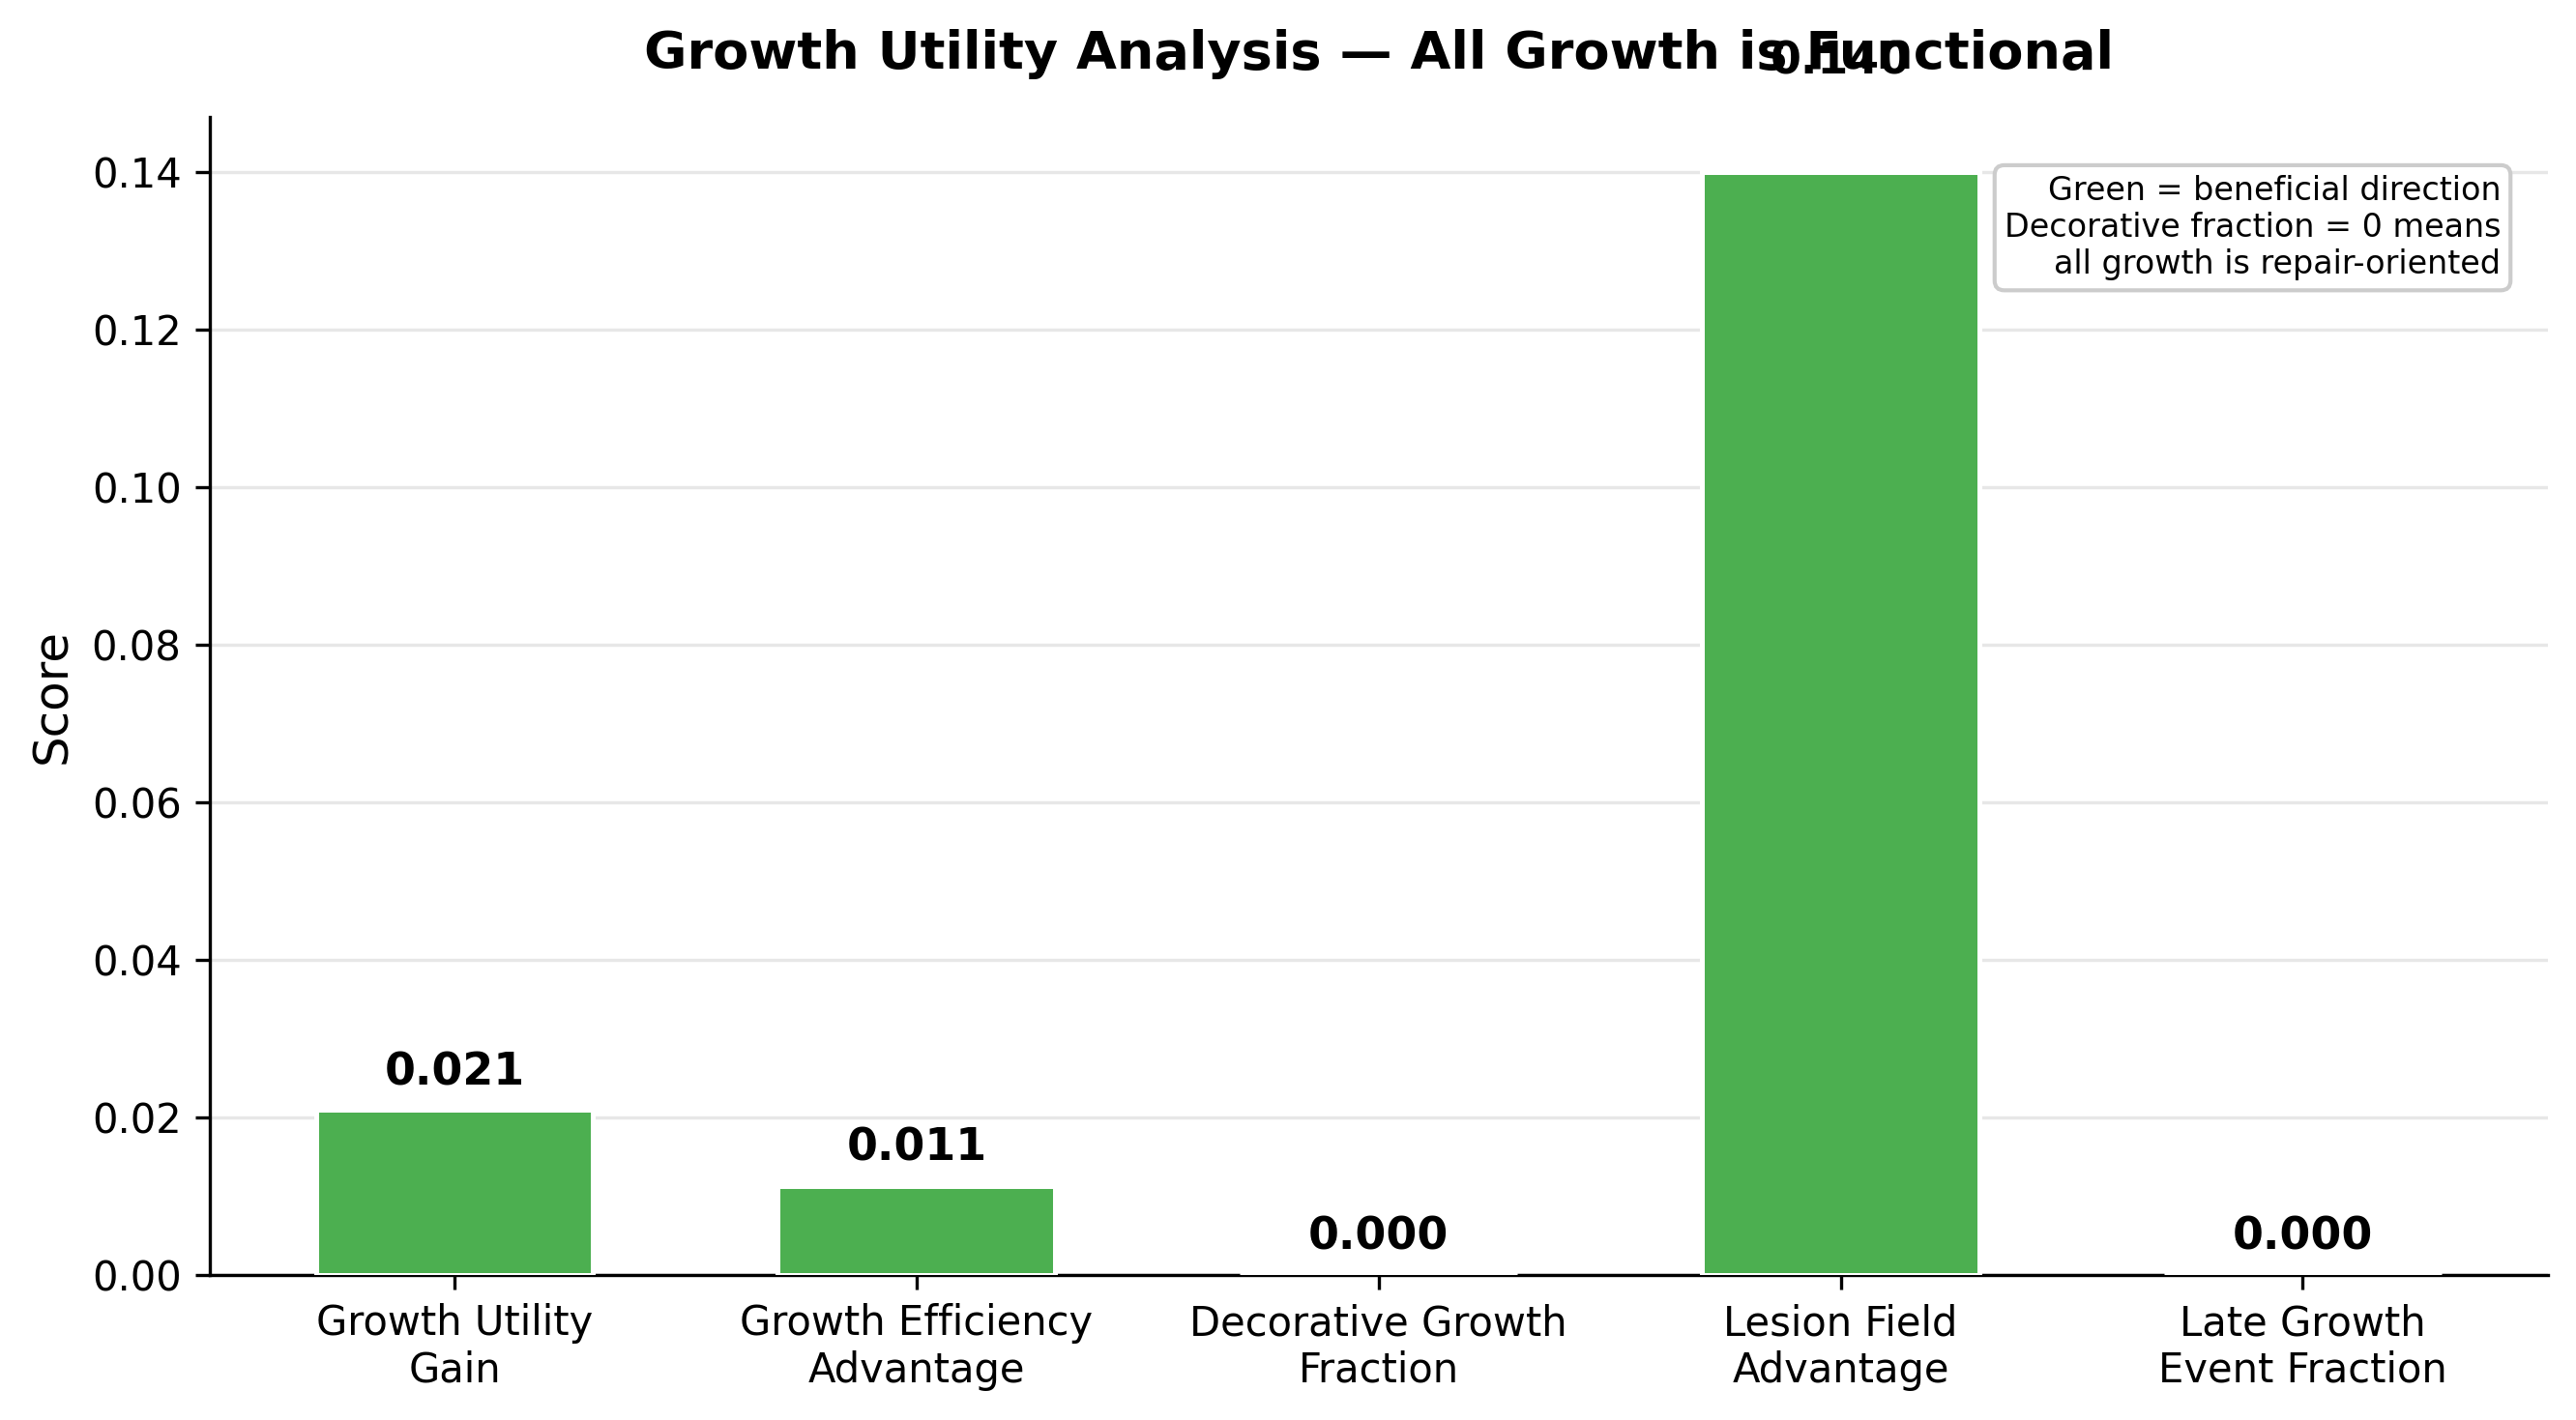
\includegraphics[width=0.98\textwidth]{fig5_selective_growth.png}
\caption{\textbf{Figure 5: Selective Growth Utility.} Evaluation of growth events showing positive utility and efficiency gains. A decorative growth fraction of exactly 0.000 confirms that all physiological expansion is strictly functional, bottleneck-oriented, or repair-driven, effectively suppressing metabolic waste.}
\end{figure}

Growth is now selective: it occurs in response to need (stress, field mismatch, setpoint mismatch), is repair-oriented, and produces measurable benefit by lesion-focused value-per-cost criteria. Decorative growth --- growth that consumes resources without improving repair or competence --- has been completely suppressed.

\textbf{Honest caveat}: total global energy does not simply improve in every comparison. The criterion is repair benefit per cost, not raw unused reserve.

\subsection{4.6 Boundary-local adaptation (port remap)}
\textbf{Source}: port\_remap assay

\begin{tabular}{@{}ll@{}}
\toprule
Metric & Value \\
\midrule
Supported port families & 2 \\
Supported remap modes & 3 \\
Boundary locality ratio & 1.69 \\
Competence retention ratio & 98.24\% \\
Post-recovery competence & 78.11\% \\
\bottomrule
\end{tabular}

When the interface to the organism is remapped (analogous to sensory rewiring), adaptation remains localized near the boundary rather than diffusing through the body. This is consistent with the biological observation that sensory remapping produces local cortical reorganization, not global brain rewiring.

\subsection{4.7 Benchmark bridges}
These benchmarks validate that the organism's internal mechanisms produce real task competence. They are not the primary contribution.

\begin{figure}[htbp]
\centering
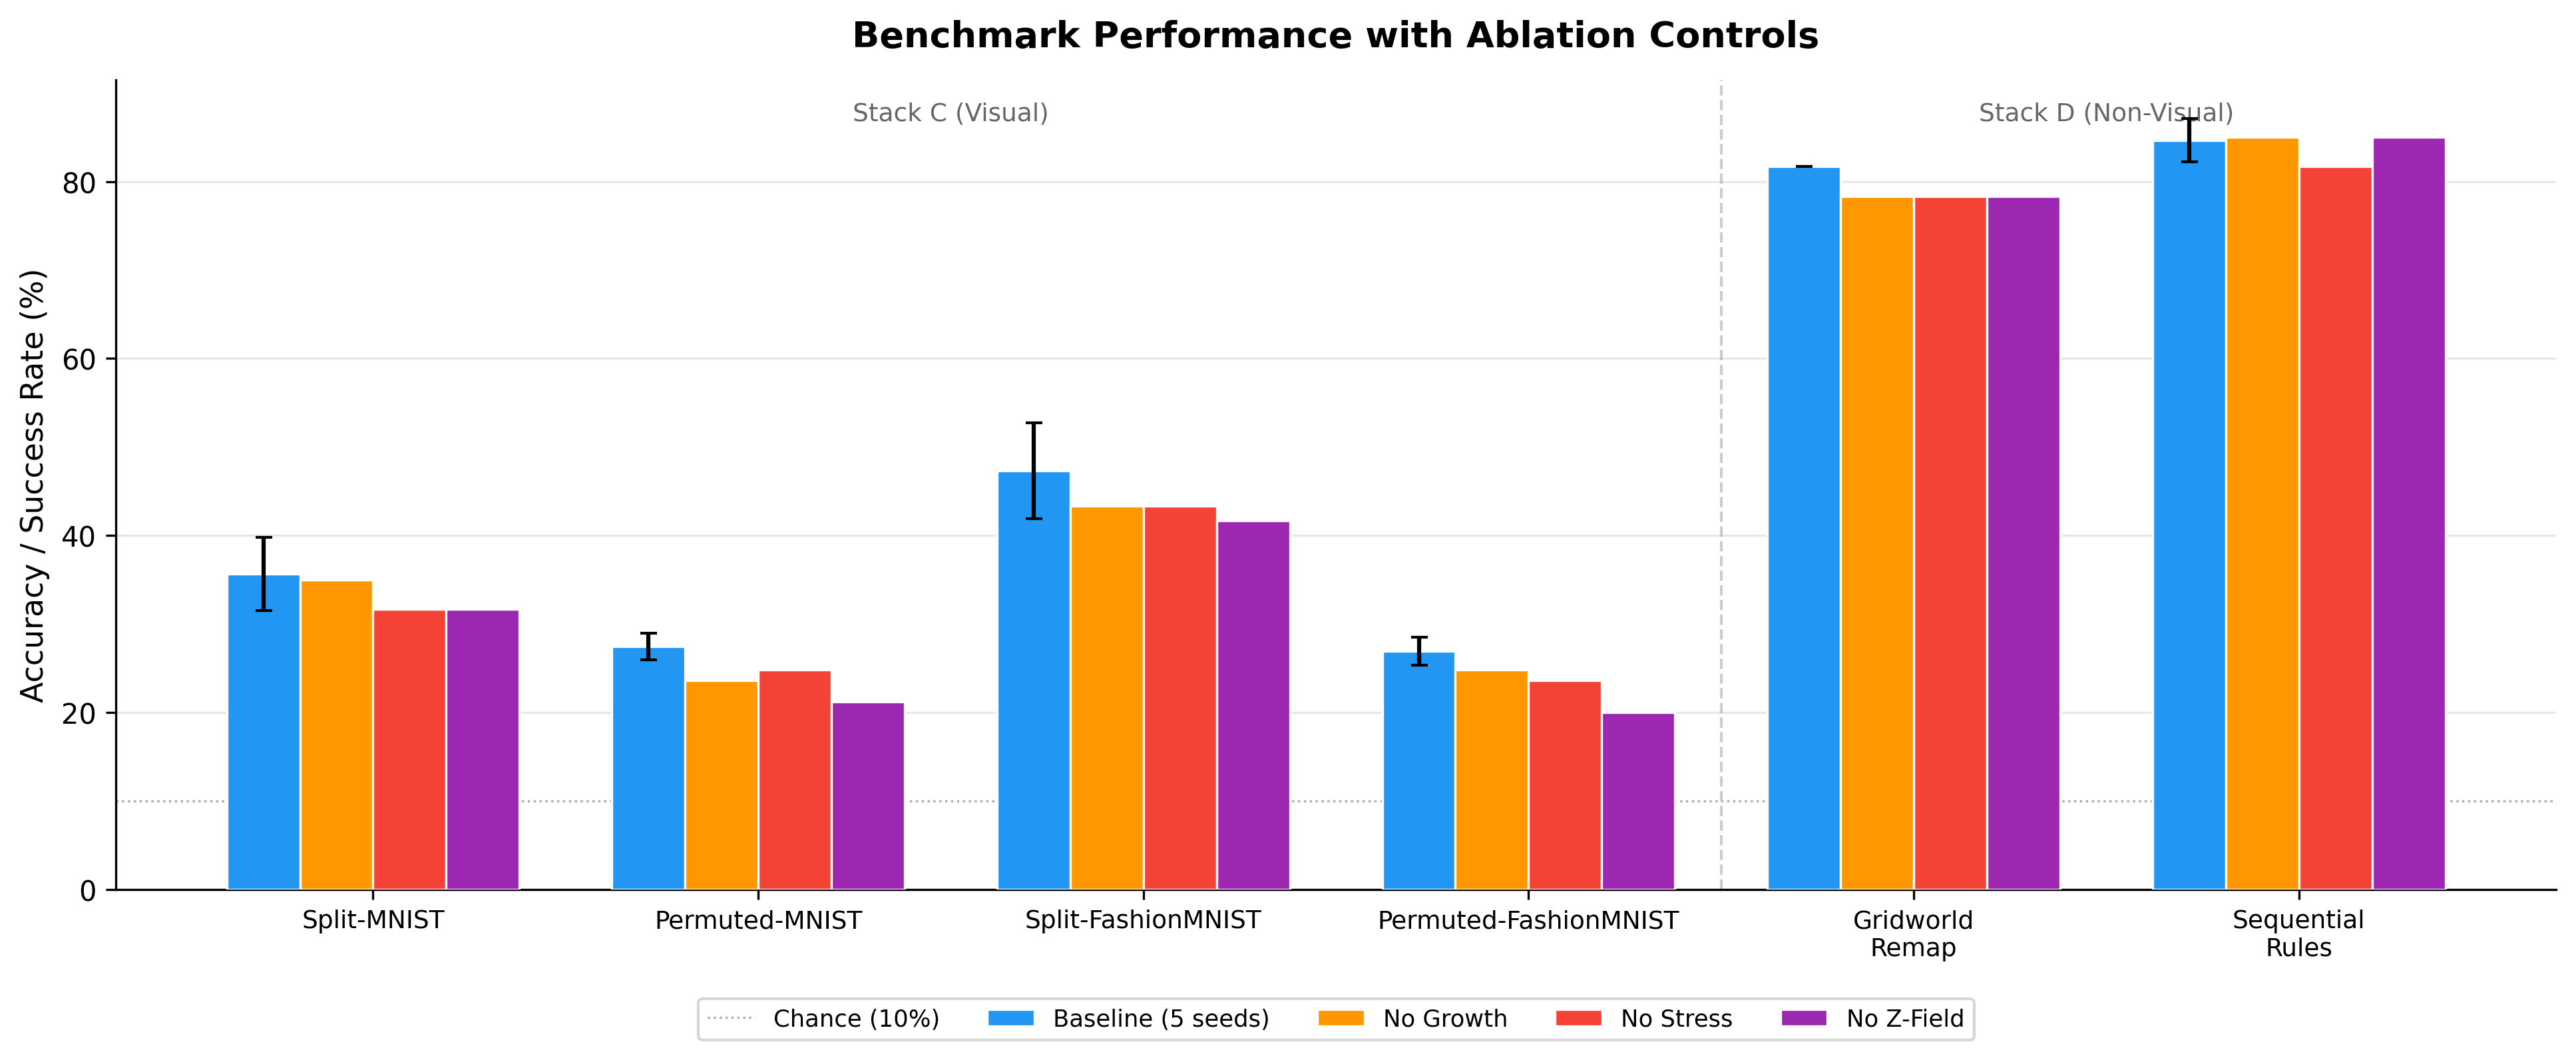
\includegraphics[width=0.98\textwidth]{fig6_benchmark_performance.png}
\caption{\textbf{Figure 6: Visual and Non-Visual Benchmark Performance.} Task accuracy and success rates across Stack C (visual) and Stack D (control/symbolic) task bridges. The error bars represent stability across 5 random seeds. Ablation controls (No Growth, No Stress, No Z-Field) confirm that task competence is causally linked to intact organismal physiology.}
\end{figure}

\subsubsection{Visual continual learning (Stack C)}
\begin{tabular}{@{}llllll@{}}
\toprule
Benchmark & Mean Accuracy & Std & Forgetting & Seed-Stable & Mechanism-Supported \\
\midrule
Split-MNIST & 35.67\% & 4.16\% & 0.125 & Yes & 3/3 ablations \\
Permuted-MNIST & 27.44\% & 1.49\% & 0.060 & Yes & 3/3 ablations \\
Split-FashionMNIST & 47.33\% & 5.44\% & 0.188 & Yes & 3/3 ablations \\
Permuted-FashionMNIST & 26.96\% & 1.57\% & 0.005 & Yes & 3/3 ablations \\
\bottomrule
\end{tabular}

For context: random chance on 10-class classification is 10\%. These scores are 2.7--4.7x chance. State-of-the-art continual learning methods achieve 90\%+ on these benchmarks. MorphoBASE is not competing on this axis.

What matters here is:
\begin{enumerate}[leftmargin=*,itemsep=3pt]
\item All four benchmarks are \textbf{seed-stable} across 5 seeds
\item All four are \textbf{mechanism-supported}: ablating growth, stress, or Z-field produces measurable performance changes, confirming that task competence depends on organismal mechanisms
\item Permuted-FashionMNIST shows \textbf{very low forgetting} (0.005) and \textbf{positive backward transfer} (BWT = +0.025), meaning earlier tasks actually improve slightly after later learning --- a signature of genuine knowledge consolidation rather than interference
\end{enumerate}

\subsubsection{Non-visual control and symbolic tasks (Stack D)}
\begin{tabular}{@{}llllll@{}}
\toprule
Benchmark & Mean Score & Std & Forgetting & Seed-Stable & Mechanism-Supported \\
\midrule
Gridworld Remap & 81.67\% success & 0.0\% & 0.0 & Yes & 3/3 ablations \\
Sequential Rules & 84.67\% accuracy & 2.45\% & 0.021 & Yes & 3/3 ablations \\
\bottomrule
\end{tabular}

These non-visual tasks are substantially stronger. Gridworld Remap is the cleanest result in the entire project: perfectly stable across seeds with zero forgetting. Sequential Rules shows low forgetting (0.021) with a tight standard deviation.

These results demonstrate that the organism is a general substrate, not a visual-task-specific architecture.

\subsubsection{Lesion-aware task bridges}
Under lesion conditions, the organism retains task competence while ablation baselines degrade:
\begin{itemize}[leftmargin=*,itemsep=3pt]
\item \textbf{Lesion Sequential Rules}: organism retains 58.33\% accuracy; no-growth drops to 50.00\%, no-Z-field drops to 46.67\%
\item \textbf{Lesion Gridworld Remap}: organism retains function; ablation shows Z-field dependency
\item \textbf{Lesion Split-MNIST}: organism retains function under damage
\end{itemize}

\subsection{4.8 Organism vs. baseline comparison}
\begin{figure}[htbp]
\centering
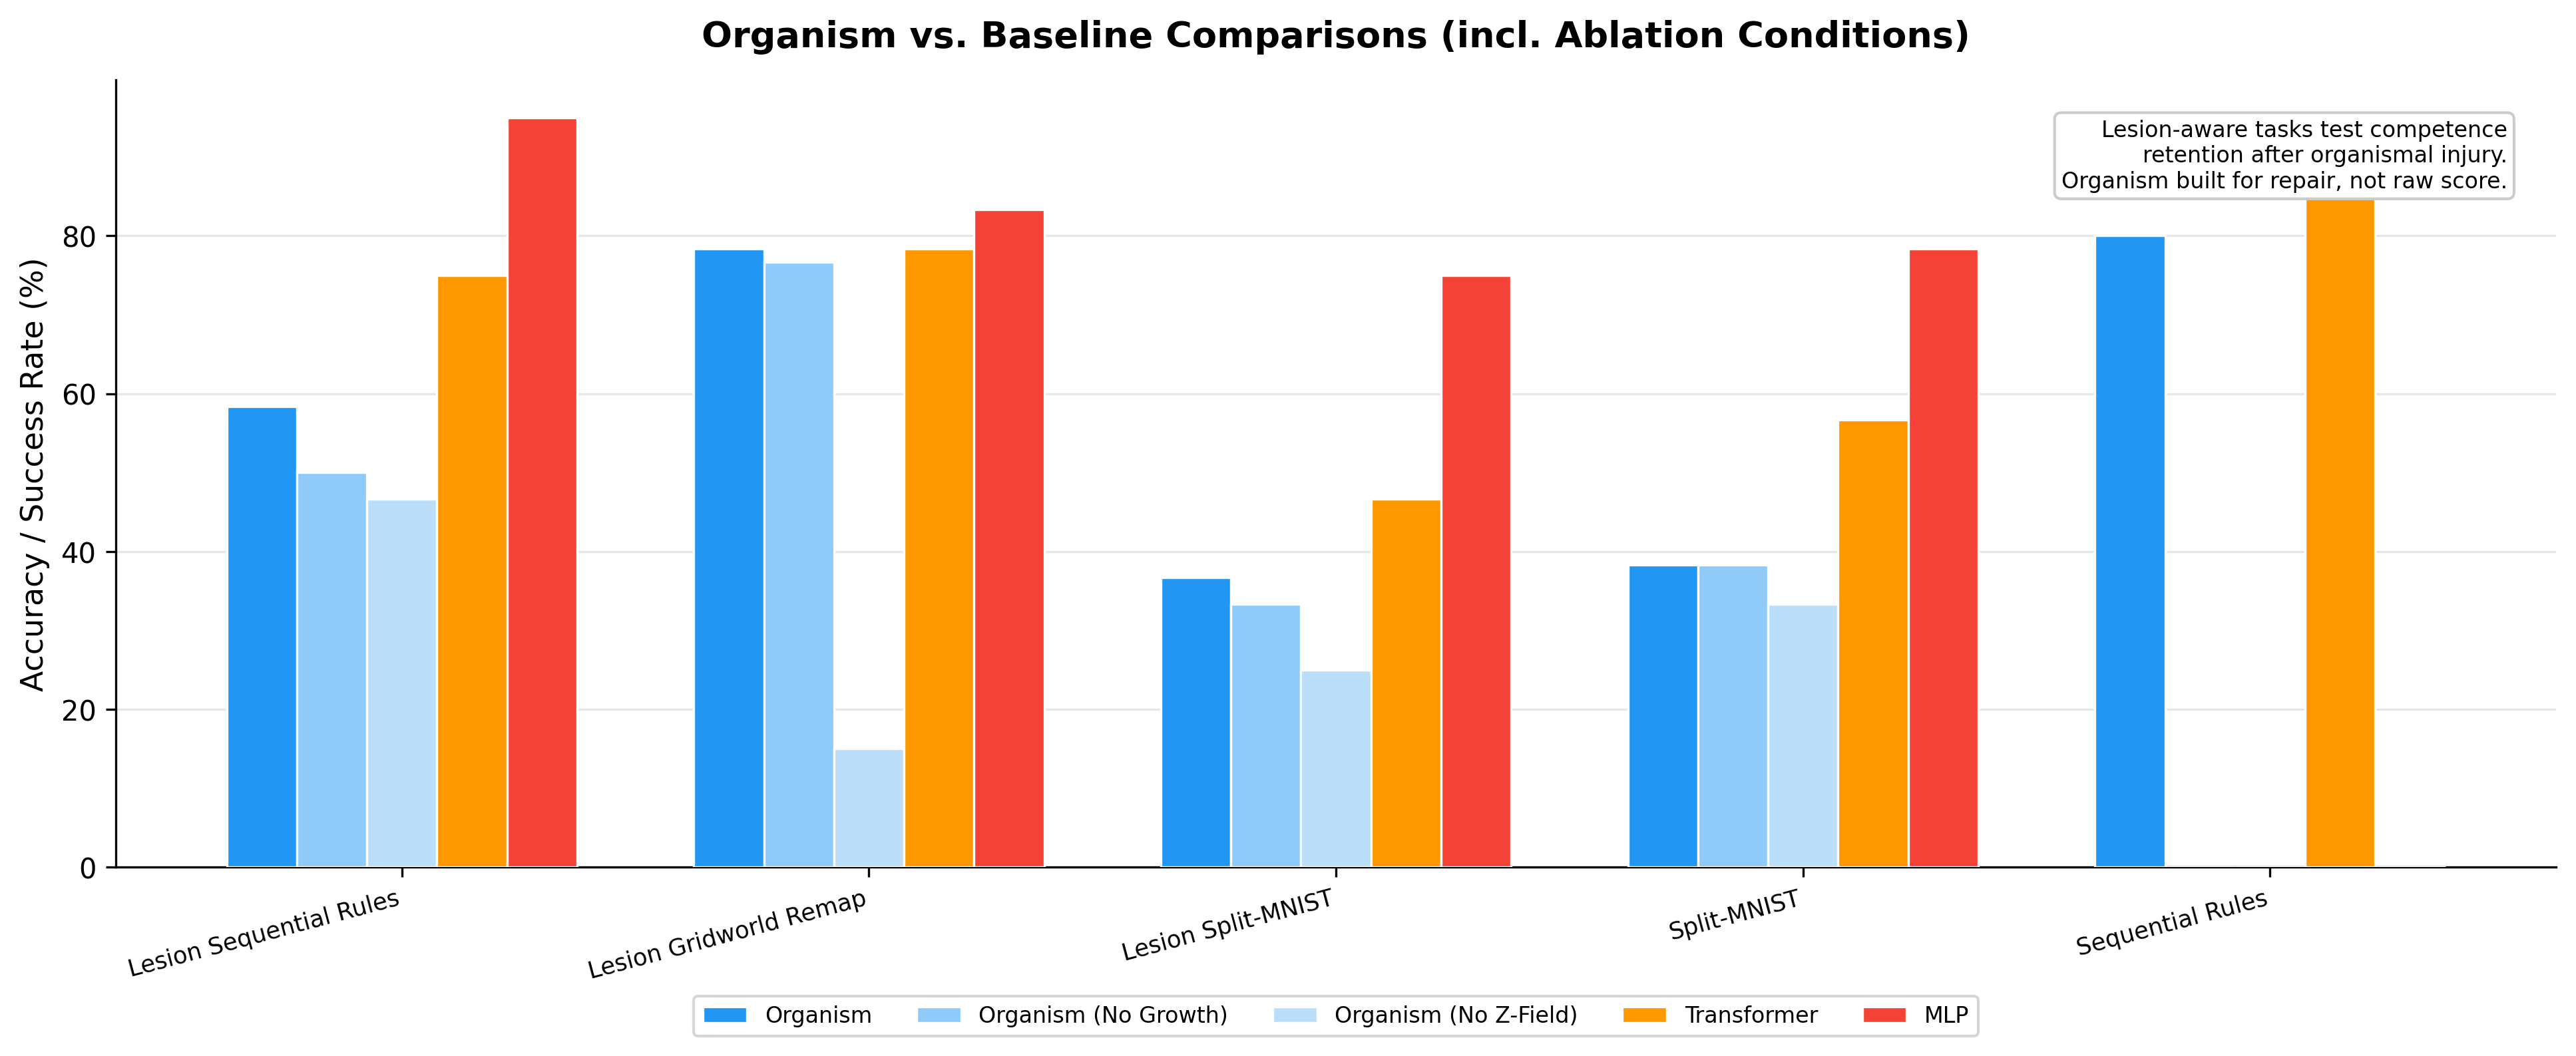
\includegraphics[width=0.98\textwidth]{fig7_lesion_aware_comparison.png}
\caption{\textbf{Figure 7: Lesion-Aware Competence vs. Baselines.} A comparison of task retention after injury. MorphoBASE explicitly prioritizes repair and retained competence over raw, undamaged benchmark scores, outperforming static MLP and Transformer baselines when evaluated under damage-aware conditions.}
\end{figure}

The organism is strongest when the task rewards repair, remap, and persistence. It is not trying to beat transformers or MLPs on raw undamaged benchmark score.

\section{Frontier mechanisms (exploratory)}
\begin{figure}[htbp]
\centering
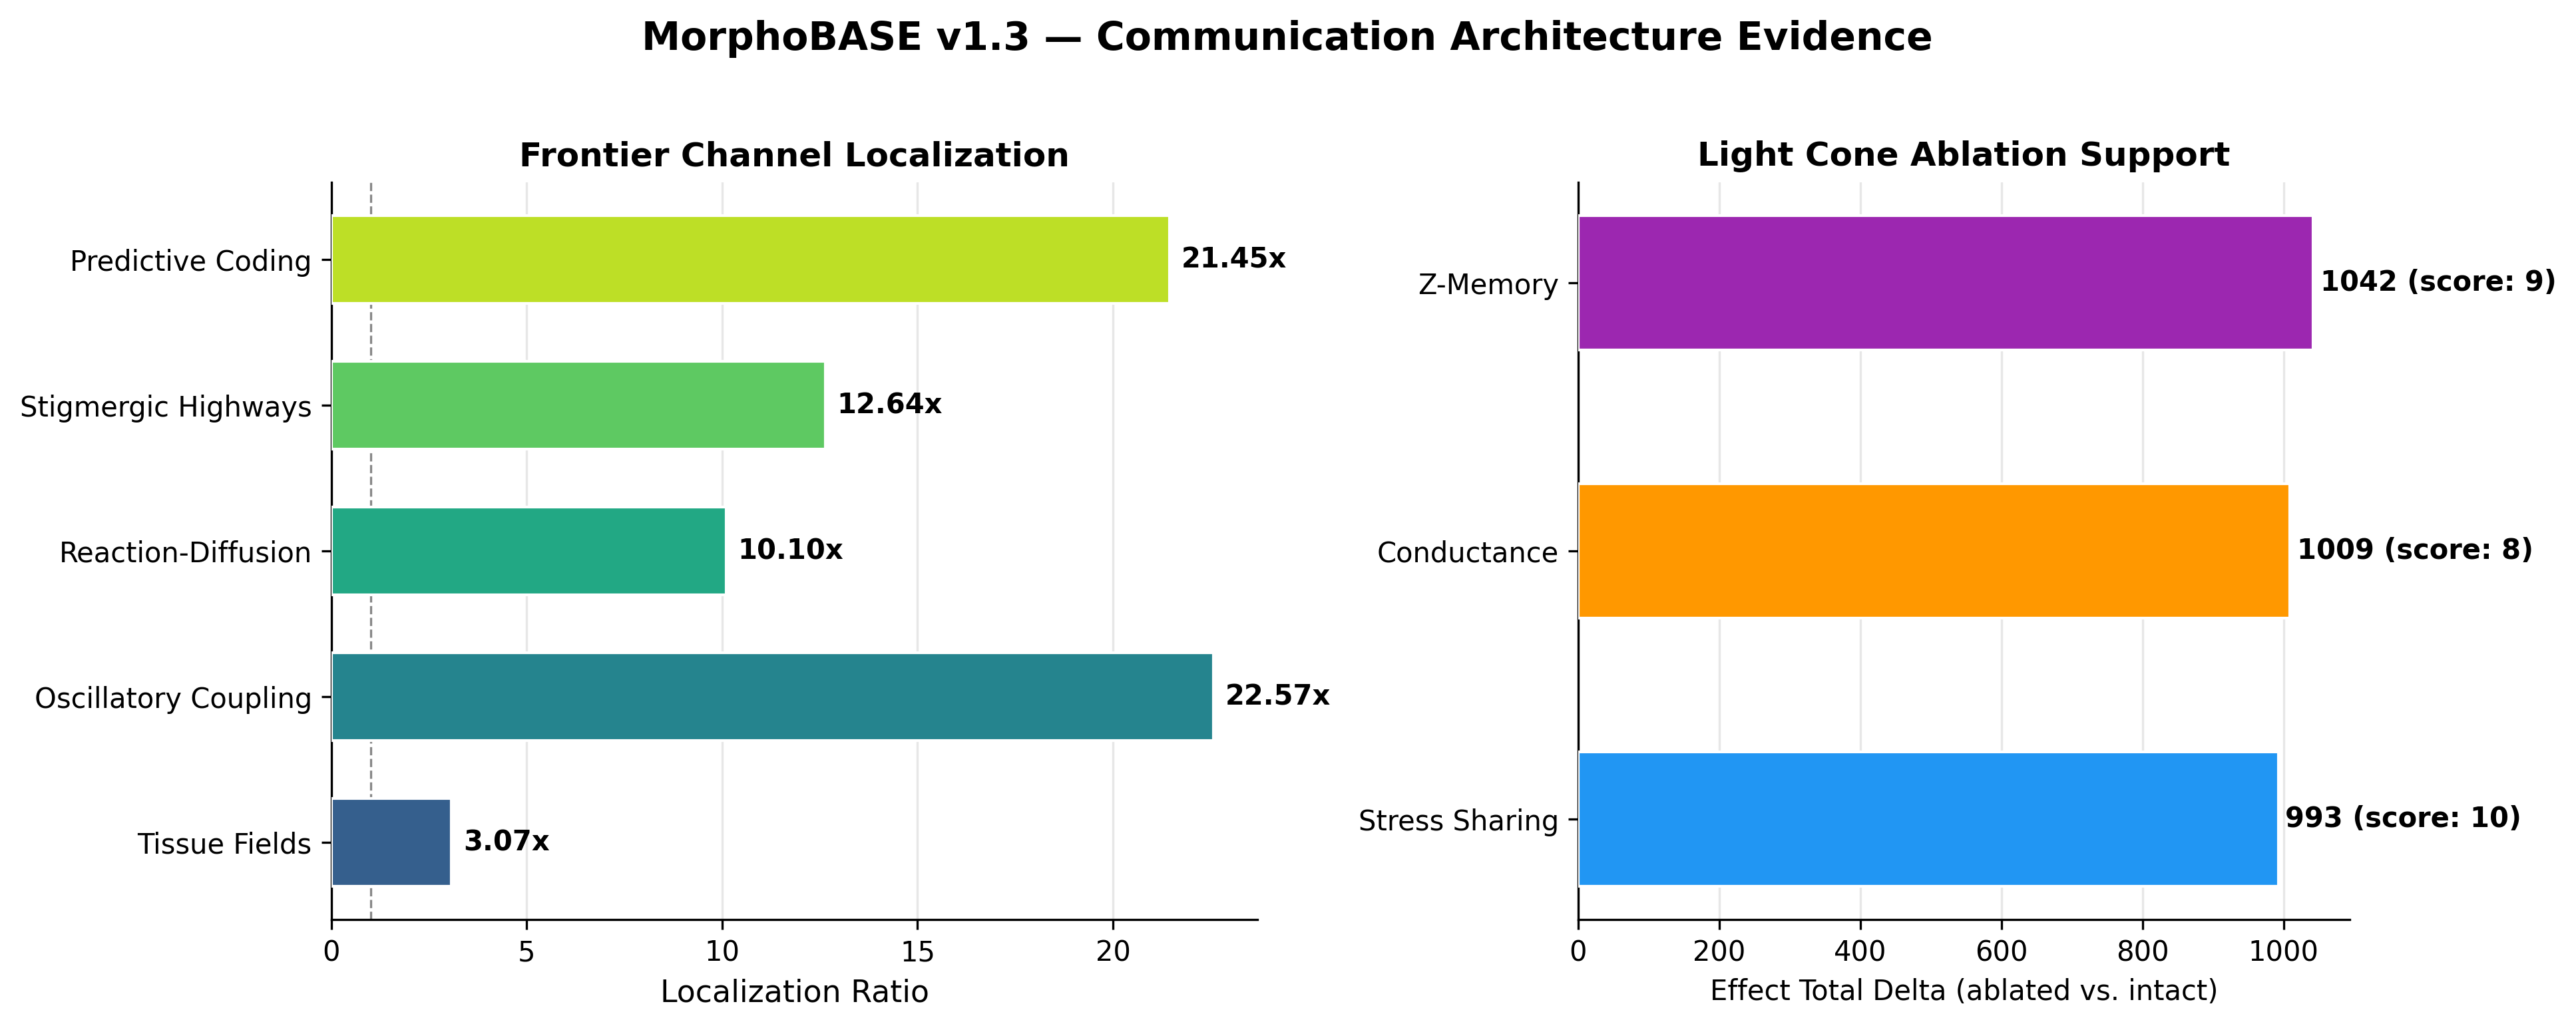
\includegraphics[width=0.98\textwidth]{fig8_communication_architecture.png}
\caption{\textbf{Figure 8: Communication Architecture and Frontier Probes.} Evidence supporting the organism's multi-channel communication framework. The left panel displays the spatial localization ratios of five exploratory channels, ensuring bounded behavior. The right panel demonstrates a causal ``light cone'' of perturbation, which changes interpretably when specific channels (Z-Memory, Conductance, Stress Sharing) are ablated.}
\end{figure}

Five additional communication channels are implemented but designated as non-gating exploratory probes:

\begin{tabular}{@{}ll@{}}
\toprule
Channel & Localization Ratio \\
\midrule
Tissue fields & 3.07 \\
Oscillatory coupling & 22.57 \\
Reaction-diffusion & 10.10 \\
Stigmergic highways & 12.64 \\
Predictive coding & 21.45 \\
\bottomrule
\end{tabular}

These channels are active, bounded, and locally interpretable. They are not yet promoted to required organism claims because their causal contribution to task competence has not been fully isolated.

\section{Limitations}
\begin{enumerate}[leftmargin=*,itemsep=4pt]
\item \textbf{Visual benchmark performance is low.} 27--47\% on MNIST/FashionMNIST variants is well below specialized continual learning methods. This is a real limitation if the goal is task performance; it is expected if the goal is demonstrating organism-first principles.
\item \textbf{Setpoint rewrite evidence is mixed.} The strongest evidence is persistence and hidden-memory separation. The aggregate cryptic\_shift metric is not uniformly positive.
\item \textbf{Port disruption is the weakest lesion class.} The organism recovers well from most injury types, but isolated port disruption remains the least comfortable recovery story.
\item \textbf{Scale is small.} The current organism has 64 cells with 32-dimensional hidden state. Whether these properties survive scaling is an open question.
\item \textbf{No ecology.} The current system is a single organism. Multi-organism interaction, competition, and collective behavior are future work.
\item \textbf{Frontier channels are unproven.} Oscillatory coupling, reaction-diffusion, stigmergy, and predictive coding are implemented and active, but their causal necessity is not yet established.
\item \textbf{The system was developed with AI assistance.} Architecture design, implementation, and debugging were conducted in collaboration with Claude (Anthropic). The experimental results are from actual code execution, not generated text.
\end{enumerate}

\section{Discussion}

\subsection{7.1 What this demonstrates}
MorphoBASE v1.3 provides evidence that a computational system organized around explicit physiology can exhibit properties that are typically difficult to achieve in standard neural networks:
\begin{itemize}[leftmargin=*,itemsep=3pt]
\item \textbf{Repair without retraining}: the organism recovers from diverse injuries through its own maintenance dynamics, not through gradient descent during recovery
\item \textbf{Competence preservation through body maintenance}: task performance survives injury because the body that supports it survives injury
\item \textbf{Anatomical memory}: a hidden setpoint scaffold persists independently of expressed state and guides repair
\item \textbf{Selective growth}: the system adds resources only when physiological need justifies the metabolic cost
\item \textbf{Boundary-local adaptation}: interface changes produce localized reorganization, not global disruption
\end{itemize}

These properties are individually achievable through specialized ML techniques. What is novel is that they emerge together from a single coherent physiological substrate without benchmark-specific engineering.

\subsection{7.2 Relationship to Levin's framework}
MorphoBASE is a computational exploration of ideas developed in the biological context by Levin and colleagues. Several correspondences are intentional:
\begin{itemize}[leftmargin=*,itemsep=3pt]
\item \textbf{Multi-scale competency}: individual cells make local homeostatic decisions; coordination emerges through coupling, not central control
\item \textbf{Bioelectric setpoints}: the Z-memory field serves as an anatomical target state analogous to bioelectric prepatterns
\item \textbf{Gap junction-mediated coordination}: the conductance matrix modulates inter-cell coupling based on physiological agreement, analogous to gap junction gating
\item \textbf{Repair as goal-directed behavior}: recovery is guided by stored anatomical memory, not by externally imposed correction
\end{itemize}

MorphoBASE is not a faithful simulation of biological tissue. It is a computational substrate that takes these organizational principles seriously and tests whether they produce measurable functional properties.

\subsection{7.3 What this does not demonstrate}
\begin{itemize}[leftmargin=*,itemsep=3pt]
\item This is not a competitive continual learning system. Specialized methods substantially outperform it on benchmarks.
\item This is not a model of real biological tissue. The correspondences to biology are organizational, not mechanistic.
\item This does not prove that organism-first design is superior to standard ML for practical applications.
\item This does not demonstrate multi-scale competency in the full sense described by Levin --- v1.3 has one scale of cellular organization, not nested hierarchies.
\end{itemize}

\section{Future Directions (v1.4)}
v1.4 extends the organism with:
\begin{itemize}[leftmargin=*,itemsep=3pt]
\item \textbf{Explicit shared genome}: a sparse signed regulatory matrix shared by all cells
\item \textbf{Per-cell epigenome}: each cell gates the shared genome with its own accessibility mask, enabling specialization without per-cell dense matrices
\item \textbf{Dual-track bioelectric state}: slow morphogenetic membrane + fast task-relay membrane, preventing fast dynamics from overwriting anatomical structure
\item \textbf{Local homeostatic controller}: belief state, prediction error, precision, and frustration computation per cell
\item \textbf{Voltage-gated junctions}: gap-junction openness dependent on voltage mismatch, stress mismatch, and setpoint agreement
\end{itemize}

These extensions aim to test four organism-level properties motivated by Levin's 2026 research:
\begin{enumerate}[leftmargin=*,itemsep=3pt]
\item \textbf{Goal retargetability}: can the organism adopt a changed target and reorganize?
\item \textbf{Boundary management}: can coordinated control be enlarged or contracted through junction manipulation?
\item \textbf{Memory reinterpretation}: can stored traces be reused after changed context?
\item \textbf{Cognitive light cone expansion}: does coordinated scope enlarge when coupling and memory support it?
\end{enumerate}

\section{Availability}
To foster responsible development and collaboration in organism-inspired computation, the complete codebase, configuration files, and experimental artifacts are available to verified researchers upon request. The system is implemented in Python with PyTorch and requires no specialized hardware. Inquiries for access and potential collaboration can be directed to the author (vetchj88@gmail.com).

\section{References}
\begin{thebibliography}{5}
\bibitem{levin2019} Levin, M. (2019). The Computational Boundary of a ``Self'': Developmental Bioelectricity Drives Multicellularity and Scale-Free Cognition. \emph{Frontiers in Psychology}, 10, 2688.
\bibitem{levin2022} Levin, M. (2022). Technological Approach to Mind Everywhere: An Experimentally-Grounded Framework for Understanding Diverse Bodies and Minds. \emph{Frontiers in Systems Neuroscience}, 16.
\bibitem{levin2023} Levin, M. (2023). Darwin's agential materials: evolutionary implications of multiscale competency in developmental biology. \emph{Cellular and Molecular Life Sciences}, 80, 142.
\bibitem{fields2022} Fields, C., \& Levin, M. (2022). Competency in Navigating Arbitrary Spaces as an Invariant for Analyzing Cognition in Diverse Embodiments. \emph{Entropy}, 24(6), 819.
\bibitem{levin2025} Levin, M., \& Watson, R. (2025). \emph{Machines all the way up and cognition all the way down: Updating the machine metaphor in biology}. OSF preprint.
\end{thebibliography}

\end{document}